\section{Metodologia}


\begin{frame}
    
    \centering
    \color{blue_theme}\huge{{Metodologia}}

\end{frame}




\begin{frame}{Soluções existentes}


    
        \begin{itemize}
            \item Busca de dispositivos com as seguintes propriedades:
                \begin{itemize}
                    \item Leitura de umidade e temperatura;
                    \item Comunicação sem fio;
                    \item Opção de alimentação por bateria;
                \end{itemize}
            
            \item Análise de custo e propriedades de soluções existentes.
        \end{itemize}
    
    
	
    \end{frame}
    
    
    \begin{frame}
    
            \begin{table}[!h]\label{tab:dataloggers_novos}
        	
        	\captionsetup{width=8cm}%Deixe da mesma largura que a tabela
        	\caption{\textit{Dataloggers: Preços e Mercados}}%
        % 	\begin{threeparttable}
        	\resizebox{\textwidth}{!}{
        	
        		\begin{tabular}{cccccc}
        			\toprule
                    % \hline
        			Modelo & Fabricante & Preço (R\$) & Mercado & Nível de Proteção & Interface sem Fio \\
        			\midrule \midrule
                    RCW-360        & Elitech            &  1.499,00 & Nacional    & IP64/IP65 & WiFi \\
                    EL-WiFi-TH     & Lascar Electronics &  1.305,14 & Estrangeiro & IP55  & WiFi    \\
                    TandD RTR-507B & TandD              &  2.242,57 & Estrangeiro & IP64  & Interface Própria    \\
                    160 TH         & testo              &  2.842,00 & Nacional    & IP20 & WiFi
                    \\ 
        		    \bottomrule
        		\end{tabular}%
        	
        	}
        	
        % 	\begin{tablenotes}
        	
        
        %     {%
        % 	\tiny{o autor.}%
        	    \tiny{tiny: o autor}\\
        	
        %     }
        % 	\end{tablenotes}
            % \end{threeparttable}
            \end{table}
    
            \begin{table}[!h]\label{tab:dataloggers_novos_propriedades}
        	
        	\captionsetup{width=7cm}%Deixe da mesma largura que a tabela
        	\caption{\textit{Dataloggers: Propriedades}}%
        	\resizebox{\linewidth}{!}{
        % 	\IBGEtab{}{%
        		\begin{tabular}{ccccccc}
        			\toprule
        			Modelo & Dimensões & Autonomia & Faixa de Leitura (ºC) & Precisão (ºC) & Umidade Relativa (\%) & Precisão(\%)\\
        			\midrule \midrule
                   RCW-360        & Não informado   & 3 meses       & -35 a 80 & 0,5 & 0 a 99 & 5    \\
                   EL-WiFi-TH     & 82 x 70 x 23 mm & 6 meses       & -20 a 60 & 0,3 & 0 a 100 & 2    \\
                   TandD RTR-507B & 62 x 47 x 19 mm & 10 meses      & -25 a 70 & 0,3 & 0 a 99  & 2,50 \\
                   160 TH         & 76 x 64 x 22 mm & Não informado & -30 a 50 & 0,1 & 0 a 100 & 2   
                    \\
        	    \bottomrule
        		\end{tabular}%
        	}
                \tiny{tiny: o autor}\\
            \end{table}
\end{frame}

\begin{frame}{Escopo de Projeto}

    \begin{block}{Escopo de projeto}
        Desenvolvimento um \textit{datalogger} de baixo custo que seja capaz de ler temperatura, umidade relativa e luminosidade de um ambiente em que ele estiver instalado. Deve ser possível que essas leituras sejam realizadas periodicamente de forma que o intervalo mínimo entre cada possa estar na casa dos segundos e devem ser armazenadas em uma mídia de armazenamento de massa removível para facilitar o resgate dessas informações posteriormente.
    \end{block}
    
\end{frame}





\begin{frame}{Especificações técnicas}

    \begin{enumerate}
        \item Possuir a capacidade de ler a temperatura do ambiente;
        \item Possuir a capacidade de ler a umidade relativa do ambiente;
        \item Possuir a capacidade de ler o nível de luminosidade do ambiente;
        \item Possuir alternativa de alimentação direta ou via bateria;
        \item Leitura de sensores via interfaces I²C, SPI e/ou UART;
        % \item Formatação dos dados lidos dos sensores para auxiliar no envio e/ou coleta;
        \item Persistir os dados em um cartão SD para facilitar a recuperação manual dos dados coletados;
        \item Persistência dos dados coletados por no mínimo 45 dias;
        % \item Interface de comunicação via rádio LoRa;
        % \item Envio periódico dos dados guardados via LoRaWan;
        \item Possuir interface de interação com o usuário;
        % \item Permitir a configuração da taxa de amostragem das variáveis lidas;
        \item Permitir o envio de dados coletados via interface de comunicação sem fio;
    \end{enumerate}
    
\end{frame}


\begin{frame}{Arquitetura de Hardware}
    
     \begin{itemize}
     \item Unidade de processamento;
     \item Sensor de luminosidade;
     \item Sensor de temperatura; 
     \item Sensor de umidade;
     \item Unidade de alimentação;
     \item Unidade de interface de usuário;
    %  \item Unidade de interface de comunicação USB;
     \item Unidade de leitura e escrita de dados em cartão SD;
     
    
      \end{itemize}
 \end{frame}
      
\begin{frame}{Arquitetura de Hardware}

    \begin{figure}
        \centering
        \caption{Diagrama de blocos.}
        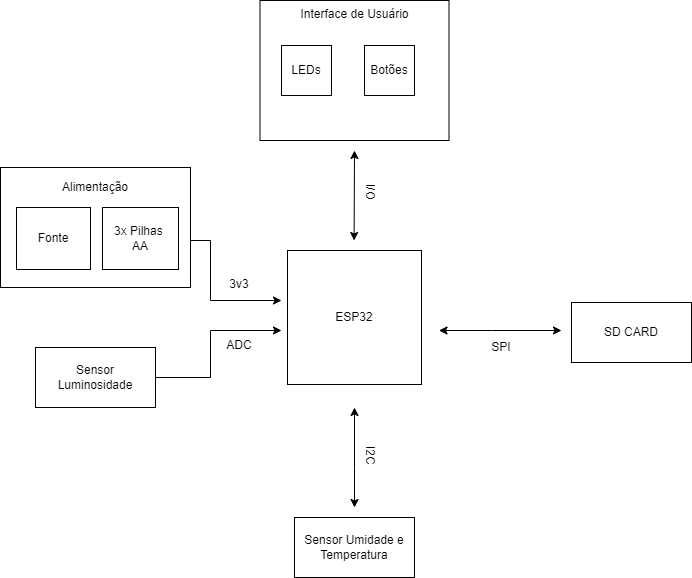
\includegraphics[scale=0.3]{figuras/cap3/datalogger_tcc.png}
        \source{Elaborado pelo autor (2022)}
        \label{fig:block_diagram}
    \end{figure}
    
\end{frame}


\begin{frame}{Seleção de Componentes}

    \begin{block}{Critérios}
        Foram definidos alguns critérios para se escolher um componente:
        
        \begin{enumerate}
            
            \item Tempo de suporte de ciclo de vida maior 10 anos p/ componentes ativos;
            \item Selecionar componentes passivos com propriedades que facilitem sua substituição;
            \item Possuir mais de uma solução para cada componente passivo;
            
        \end{enumerate}
    
        
    \end{block}

\end{frame}

\begin{frame}{Microcontrolador}

\only<1>{

    \framesubtitle{Definição}

    \begin{columns}
            
        \column{0.4\textwidth}
        \justify 
        \begin{itemize}
            \item ESP32-S3-WROOM-1-N8
            \begin{itemize}
                \item Baixo custo unitário;
                \item 8MB de \textit{Flash} e 36 GPIOs;
                \item Wi-Fi 2.4GHz e BLE Radio;
                \item ADC 10-bits;
                \item 12 anos de suporte de ciclo de vida.
                % \item 
            \end{itemize}
        \end{itemize}
        
        \column{0.6\textwidth}
        \justify
        \begin{figure}
            % \centering
            \caption{Diagrama de blocos do módulo}
            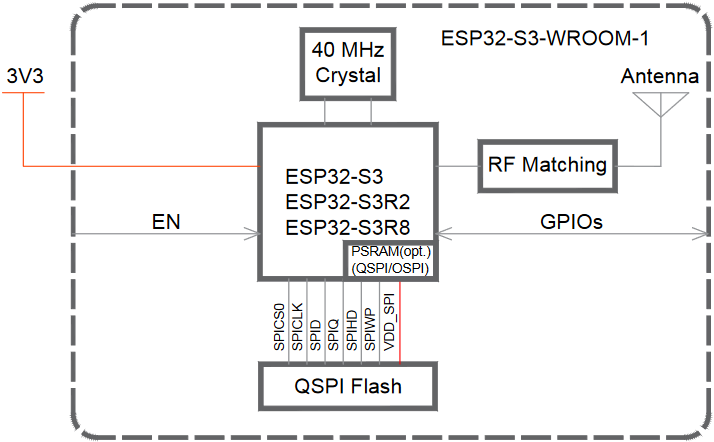
\includegraphics[scale=0.35]{figuras/cap3/modulo_block_diagram.png}
            \source{Espressif Systems}
            \label{fig:soc_esp32}
        \end{figure}
    \end{columns}
}



\only<2>{
\framesubtitle{Esquemático}

    \begin{figure}
        \centering
        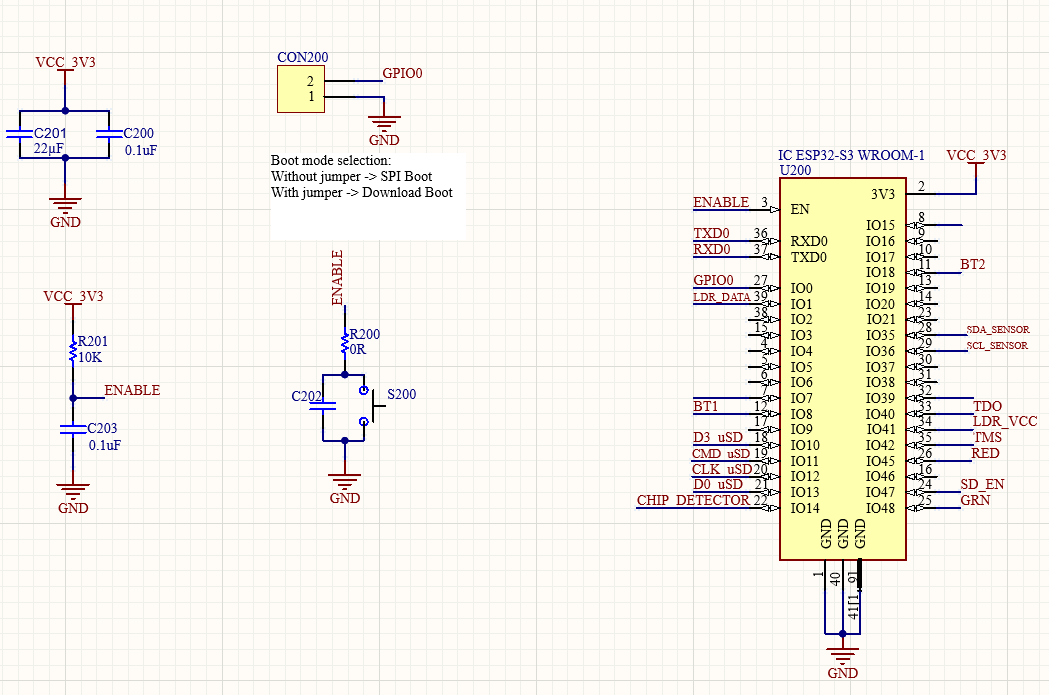
\includegraphics[width=0.85\textwidth]{figuras/cap3/esquematicos/controller.png}
        \source{Elaborado pelo autor}   
    \end{figure}
}





\end{frame}

\begin{frame}{Sensores}

    \only<1>{
        \framesubtitle{HDC1080}
        \begin{columns}
                \column{0.45\textwidth}
                \centering
                \begin{itemize}
                    \item TI HDC1080
                    \begin{itemize}
                        \item $\pm$2\% de precisão de umidade relativa;
                        \item $\pm$0.2 °C precisão de temperatura;
                        \item 1.3 $\mu$A p/ leitura e 100 nA hibernação;
                        % \item Interface I²C
                    \end{itemize}
                \end{itemize}
                
                \column{0.55\textwidth}
                \centering

                \begin{figure}
                    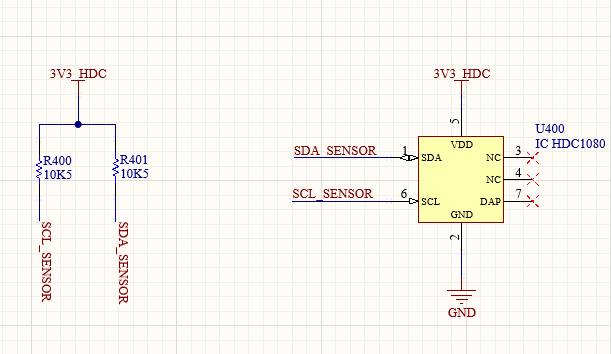
\includegraphics[width=\textwidth]{figuras/cap3/esquematicos/temp_sensor.png}
                \end{figure}
                
                
        \end{columns}

    }




    \only<2>{

        \framesubtitle{LDR}
        \begin{columns}
            \column{0.5\textwidth}

            \begin{itemize}
                \item \textit{Light Dependant Resistor} (LDR)
                \begin{itemize}
                    \item Baixo custo;
                    \item 10 a 10.000 lux;
                    \item Necessita de ADC;
                \end{itemize}
            \end{itemize}
            
            \column{0.5\textwidth}
                       
                \begin{figure}
                    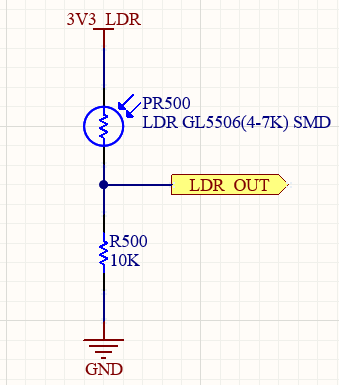
\includegraphics[width=0.7\textwidth]{figuras/cap3/esquematicos/light_sensor.png}
                \end{figure}
            
            
            
            
        \end{columns}

    }

    
\end{frame}

\begin{frame}{Interface de usuário e suporte MicroSD}


    \only<1>{
        \begin{columns}
            \column{0.45\textwidth}
                \vspace{-40pt}
                \centering
                \begin{itemize}
                    \item \textit{LEDs} e botões táteis
                    \begin{itemize}
                        \item LEDs genéricos vermelho e verde;
                        \item Dois botões táteis;
                    \end{itemize}
                
                    \vspace{50pt}
                
                    \item Suporte microSD
                
                \end{itemize}
                



                % \begin{itemize}

                
                % % \begin{itemize}
                % %     \item
                % % \end{itemize}
                % \end{itemize}


                \column{0.55\textwidth}
                \centering

                


                \begin{figure}
                    \centering
                    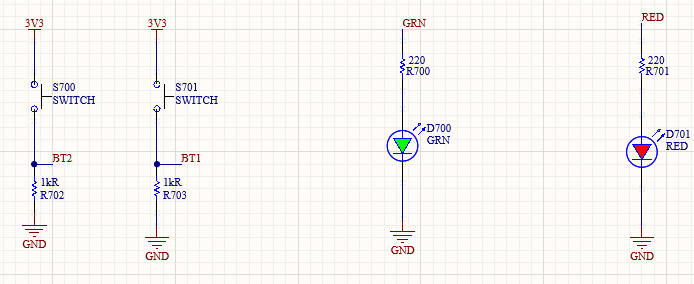
\includegraphics[width=\textwidth]{figuras/cap3/esquematicos/user_interface.png}
                    % \source{Elaborado pelo autor.}
                \end{figure}


                \begin{figure}
                    \centering
                    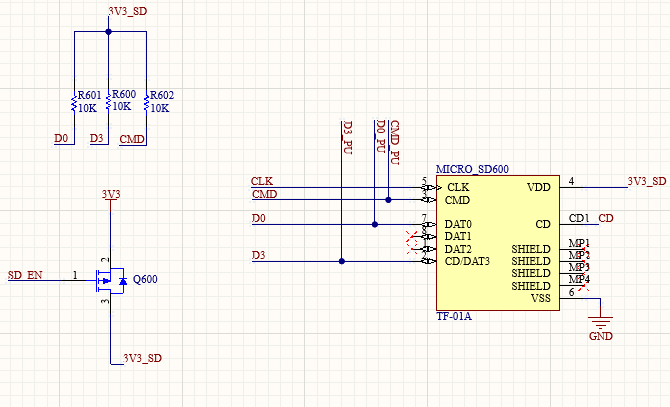
\includegraphics[width=\textwidth]{figuras/cap3/esquematicos/sdcard.png}
                    \vspace{-15pt}
                    \source{Elaborado pelo autor.}
                \end{figure}
        
        \end{columns}
    }

% \only<2>{

%     \framesubtitle{Esquemático}
%     \begin{columns}
%         \column{0.5\textwidth}
 
        
%         \column{0.5\textwidth}
                   

        
        
        
        
%     \end{columns}

% }


\end{frame}

\begin{frame}{Fonte de alimentação}

    \only<1>{
        \begin{block}{Requisitos}
            \begin{enumerate}
                \item Fornecer 3,3 V;
                \item Suportar alimentação por 4 pilhas;
                \item ``Chaveamento'' entre pilhas e alimentação direta;
            \end{enumerate}
        \end{block}
    }

% \framebreak
    \only<2>{

        % \begin{columns}
        %     \column{0.35\textwidth}
                % \vspace{3pt}
                \begin{itemize}
                    \item Circuito ``chaveador'' pilha-alimentação direta:
                    \begin{itemize}
                        \item MOSFET Canal P;
                        \item Resistor 10k$\Omega$;
                        \item Diodo \textit{schottky};
                    \end{itemize}
                    \item \textit{Schottky} ON NSR0320MW2T1
                    \begin{itemize}
                        \item Tensão direta típica: 0,3 V;
                    \end{itemize}
                    
                \end{itemize}
            % \column{0.65\textwidth}
                \vspace{-7pt}
                \begin{figure}
                    \centering
                    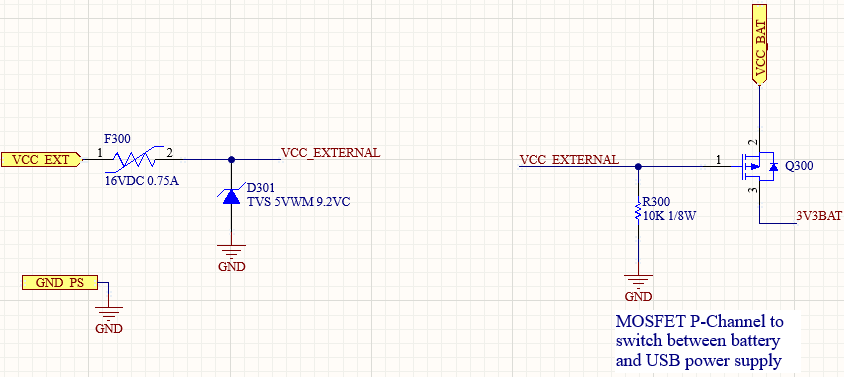
\includegraphics[width=0.8\textwidth]{figuras/cap3/esquematicos/power_1.png}
                    % \source{Elaborado pelo autor.}
                \end{figure}




        % \end{columns}

    }


% \framebreak
    
        \only<3>{        
            \begin{block}{Regulação de tensão}

            Quatro pilhas do tipo AA fornecem até 6V de tensão. É preciso reduzi-lá para 3,3 V, nível de tensão operacional dos demais componentes.

            \end{block}

            \begin{columns}
                    
                    \column{0.5\linewidth}
                    \centering
                    \begin{itemize}
                        \item Regulador Linear
                        \begin{itemize}
                            \item Baixo custo;
                            % \item Menor uso de componentes;
                            \item Baixa complexidade;
                            \item Baixa eficiência;
                            \item \textit{Step-down};
                        \end{itemize}
                    \end{itemize}
                    
                    \column{0.5\linewidth}
                    
                    \begin{itemize}
                        \item Regulador Chaveado
                        \begin{itemize}
                            \item Maior custo;
                            % \item Maior uso de componentes;
                            \item Alta complexidade;
                            \item Alta eficiência;
                            \item \textit{Step-up} ou \textit{Step-down};
                        \end{itemize}
                    \end{itemize}
                    
            \end{columns}

        }    


% \framebreak
        \only<4>{
            \begin{block}{Regulador linear \textit{low-dropout}}

            Reguladores lineares que podem regular a tensão de saída mesmo quando a tensão entrada se aproximar muito da tensão de saída.

            \end{block}

            \begin{columns}
                \column{0.45\textwidth}
                    \begin{itemize}
                        \item Diodes AP2114HA-3.3TRG1
                        \begin{itemize}
                            \item Suporta até 6,5 V de entrada;
                            \item 3,3 V fixo como saída;
                            \item Queda típica de 0,1 V;
                        \end{itemize}
                    \end{itemize}
                \column{0.55\textwidth}
                    
                    \begin{figure}
                        \centering
                        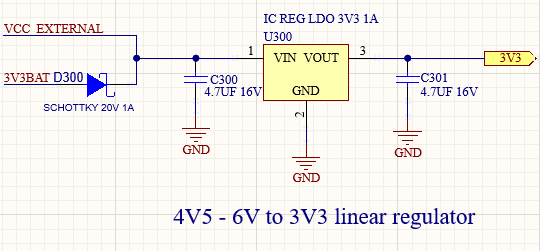
\includegraphics[width=\textwidth]{figuras/cap3/esquematicos/power_2.png}
                        \source{Elaborado pelo autor.}
                    \end{figure}   



                
            \end{columns}
            % \framebreak
        }    
\end{frame}



\begin{frame}{Design PCI}

    \only<1>{
    \begin{block}{Especificações}
    
    \begin{itemize}
        \item Dimensões aproximadas de 50x50 mm;
        \item Placa de duas camada;
    \end{itemize}
    \end{block}
    }
      
    
    % \framesubtitle{\textit{Stackup} PCI}
    \centering
    \only<2>{

    \begin{block}{\textit{Stackup PCI}}
        
        Define características e parâmetros do cobre e dielétrico de uma PCI.
    
    \end{block}
    \begin{figure}
        \centering
        
        
        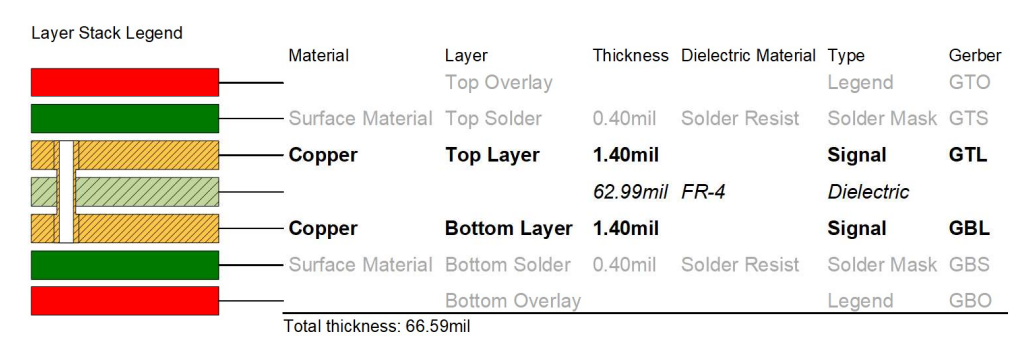
\includegraphics[width=0.7\linewidth]{figuras/cap3/pcb/pcb_stackup.png}
       
        % \includegraphics{}
        % \caption{}
        \scriptsize{Impedância típica: 50$\Omega$}
        % \caption{Particionamento Recomendado}
        \source{Elaborado pelo autor.}
        
        \label{fig:stackup_pci}
    \end{figure}
    
    }
    % \item Impedância típica - 50$\Omega$
    
    \only<3>{
    
    \framesubtitle{{Particionamento Funcional}}
    
    \begin{columns}
        \column{0.45\linewidth}
        \raggedleft
        \begin{itemize}
            \item Posição de componentes;
            \item Auxílio de roteamento;
            \item Redução EMI;
        \end{itemize}
        
        
        \column{0.55\linewidth}
        \raggedright
        \begin{figure}
            \centering
            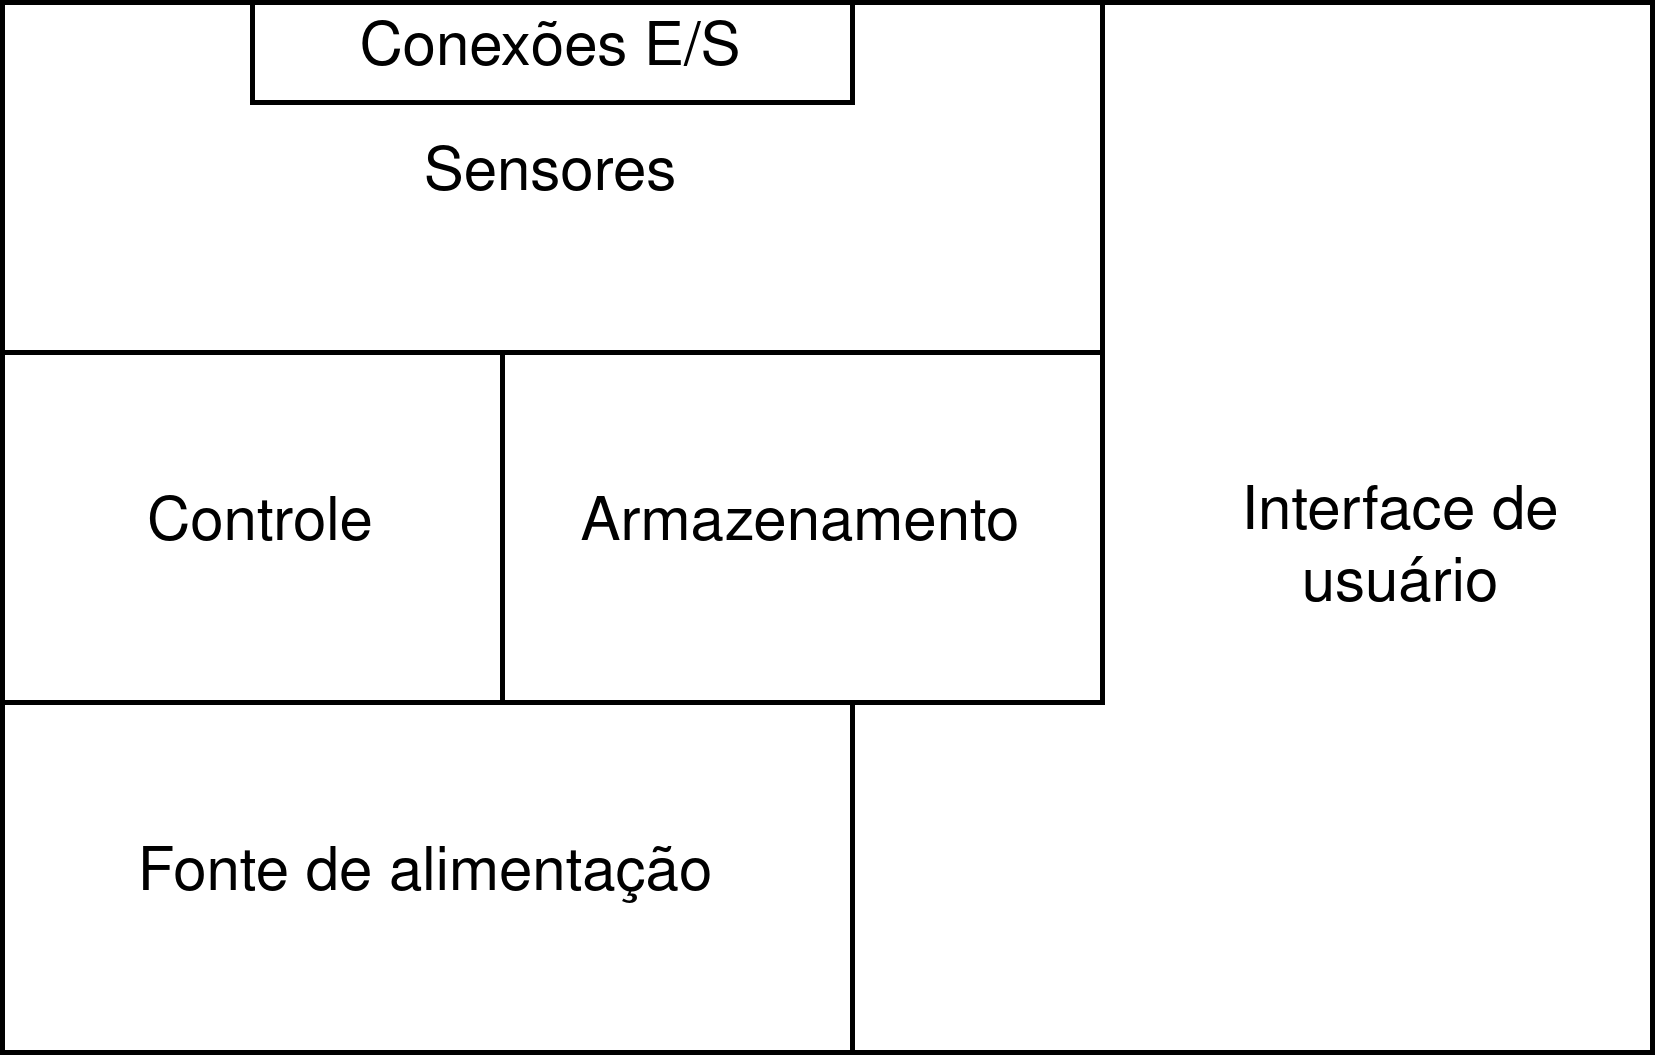
\includegraphics[width=\linewidth]{figuras/cap3/particionamento.drawio.PNG}
            % \caption{Caption}
            \source{Elaborado pelo autor.}
            \label{fig:my_label}
        \end{figure}
    
    \end{columns}

    }

    \only<4>{
    
    \framesubtitle{{Posicionamento}}
    
    \begin{figure}
        \centering
        \caption{\textit{PCB Placement}}
        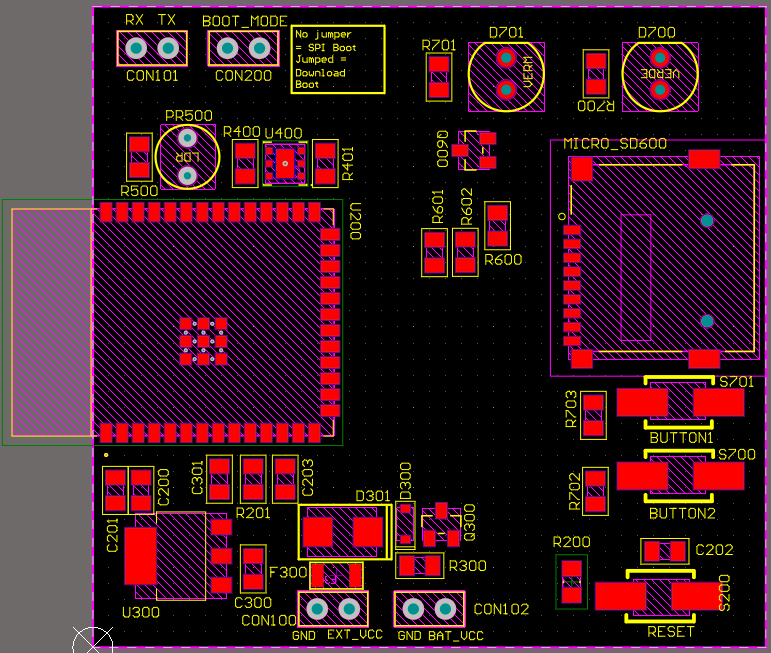
\includegraphics[width=0.6\linewidth]{figuras/cap3/pcb/pcb_no_route.png}
        \source{Elaborado pelo autor}
        \label{fig:pcb_placement}
    \end{figure}
    }

    \only<5>{

    \framesubtitle{{Roteamento}}

    \begin{columns}
        
        \column{0.4\linewidth}
        \centering
        \begin{itemize}
            \item Somente sinais inicialmente;
            \item Largura 10 mil;
        \end{itemize}
        
        \column{0.6\linewidth}
        \begin{figure}
            \centering
            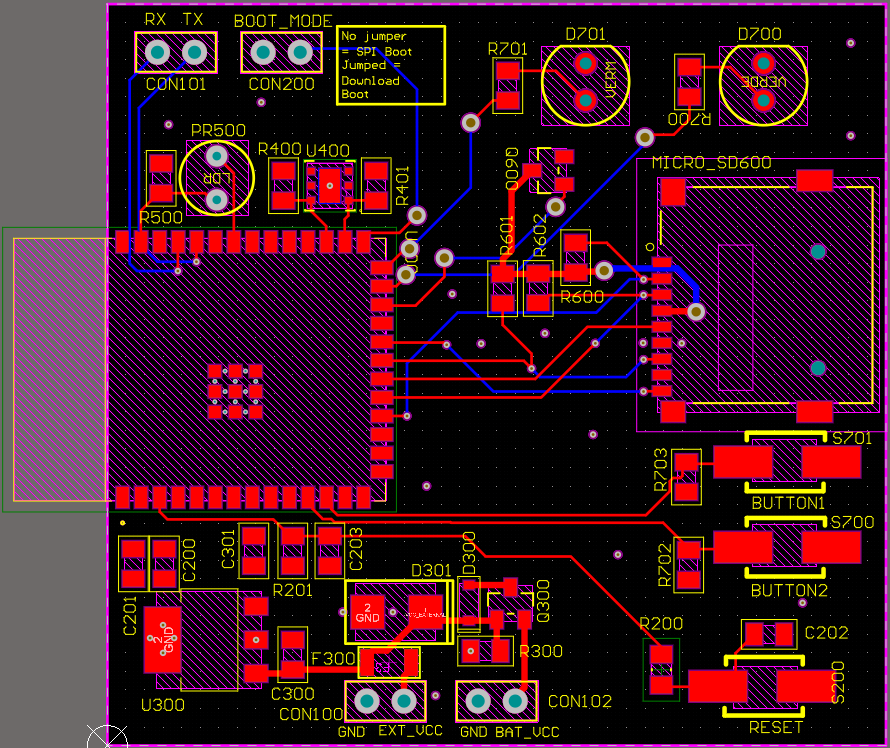
\includegraphics[width=\linewidth]{figuras/cap3/pcb/pcb_signlas_route.png}
            \source{Elaborado pelo autor}
        \end{figure}


    \end{columns}
    }

    \only<6>{

    \framesubtitle{{Roteamento}}

    \begin{columns}
        
        \column{0.4\linewidth}
        \centering
        \begin{itemize}
            \item Evita ciclos;
            \item Largura 20 mil;
        \end{itemize}
        
        \column{0.6\linewidth}
        \begin{figure}
            \centering
            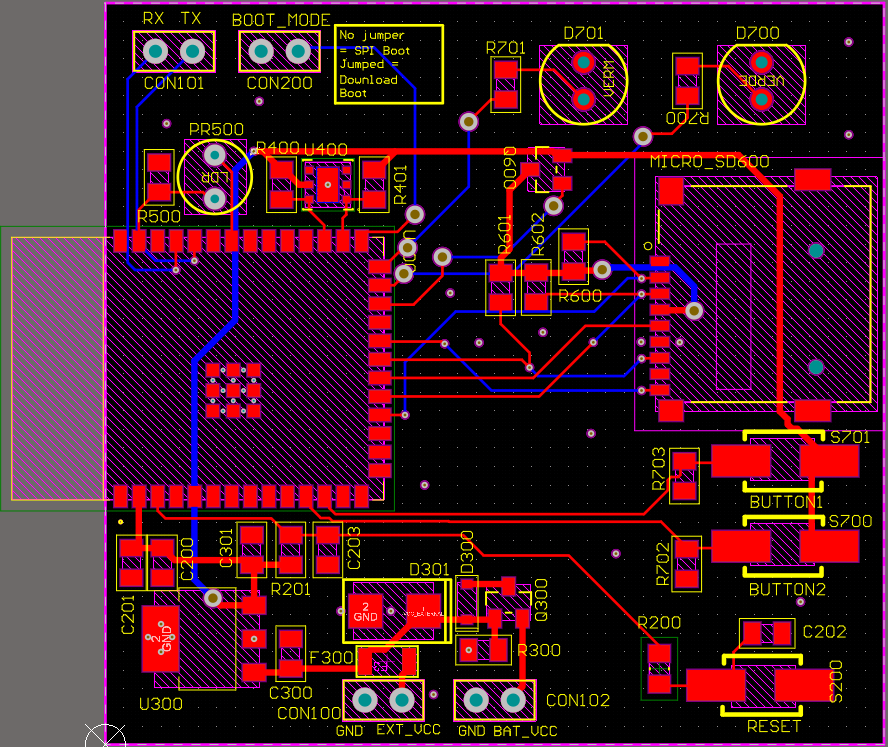
\includegraphics[width=\linewidth]{figuras/cap3/pcb/pcb_with_power.png}
            \source{Elaborado pelo autor}
        \end{figure}


    \end{columns}

    }


    \only<7>{

        \begin{block}{Plano de Terra}
            Propicia o menor caminho de retorno possível
        \end{block}

        % \vspace{10pt}

        \begin{columns}
        % \begin{figure}
            
    
            % \begin{subfigure}{0.5\linewidth}
                \column{0.45\linewidth}
                \centering
                % \vspace{3pt}
                \captionof{figure}{Top Plane}
                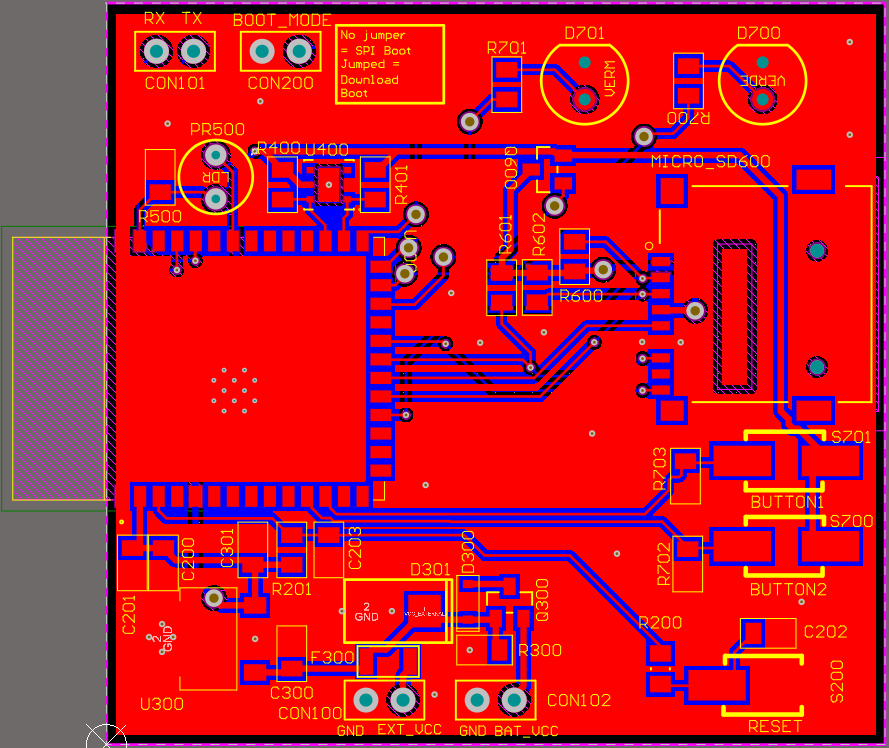
\includegraphics[width=\linewidth]{figuras/cap3/pcb/pcb_top_plane.png}
                % \source{Elaborado pelo autor}
            % \end{subfigure}   
            
            % \begin{subfigure}{0.5\linewidth}
                \column{0.45\linewidth}
                \centering
                % \vspace{3pt}
                \captionof{figure}{Bottom Plane}
                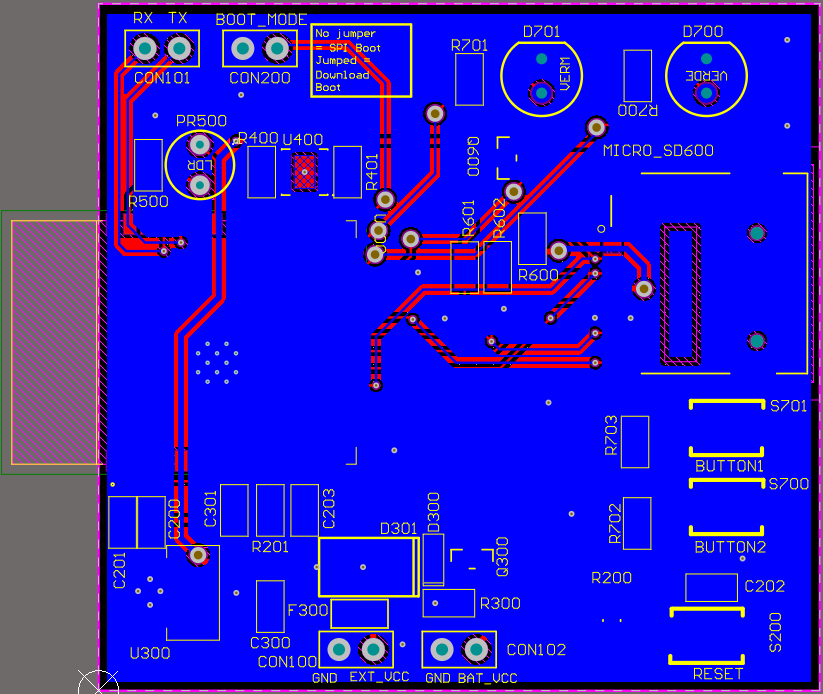
\includegraphics[width=\linewidth]{figuras/cap3/pcb/pcb_bottom_plane.png}
                % \source{Elaborado pelo autor}
                
            % \end{subfigure}

            % \source{Elaborado pelo autor}
        % \end{figure}
        \end{columns}

        \begin{figure}
            \centering
            \source{Elaborado pelo autor}
        \end{figure}

    }
    
    
    
    
    
\end{frame}
